\documentclass[a4paper,12pt]{article}
\usepackage[utf8]{inputenc}
\usepackage{authblk}
\usepackage{graphicx} 
\date{}

\begin{document}
\pagenumbering{gobble}
\title{Irene: Integrative Ranking with Epigenetic Network of Enhancers}
\author[1,3]{Qi Wang}
\author[2]{Yonghe Wu}
\author[3,4]{Roland Eils}
\author[1]{Carl Herrmann}
\affil[1]{Faculty of Biosciences, Heidelberg University, Heidelberg, Germany}
\affil[2]{Division of Molecular Genetics, German Cancer Research Center (DKFZ), Heidelberg, Germany}
\affil[3]{Division of Theoretical Bioinformatics, German Cancer Research Center (DKFZ), Heidelberg, Germany}
\affil[4]{Digital Health Center, Berlin Institute of Health (BIH) and Charité, Berlin, Germany}

\maketitle

\begin{figure}[!htb]
\centering
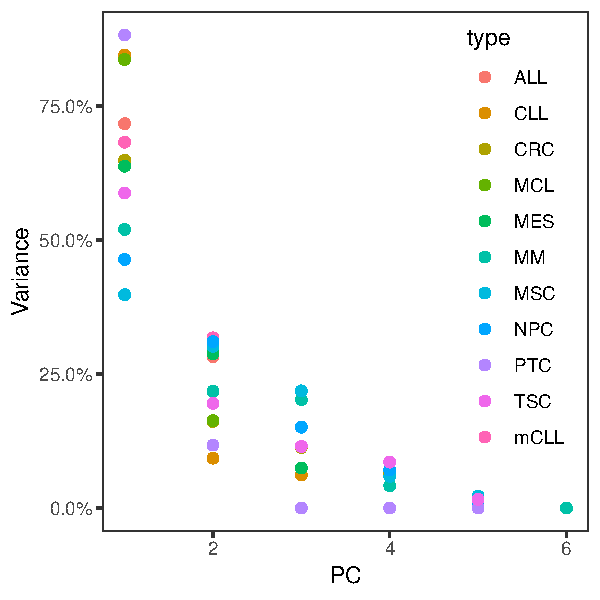
\includegraphics{figs/PCvar.pdf}
\caption{ PC1 explained $\sim 40\%-100\%$ variances. }
\label{fig:pcvar}
\end{figure}

\begin{figure}[!htb]
\centering
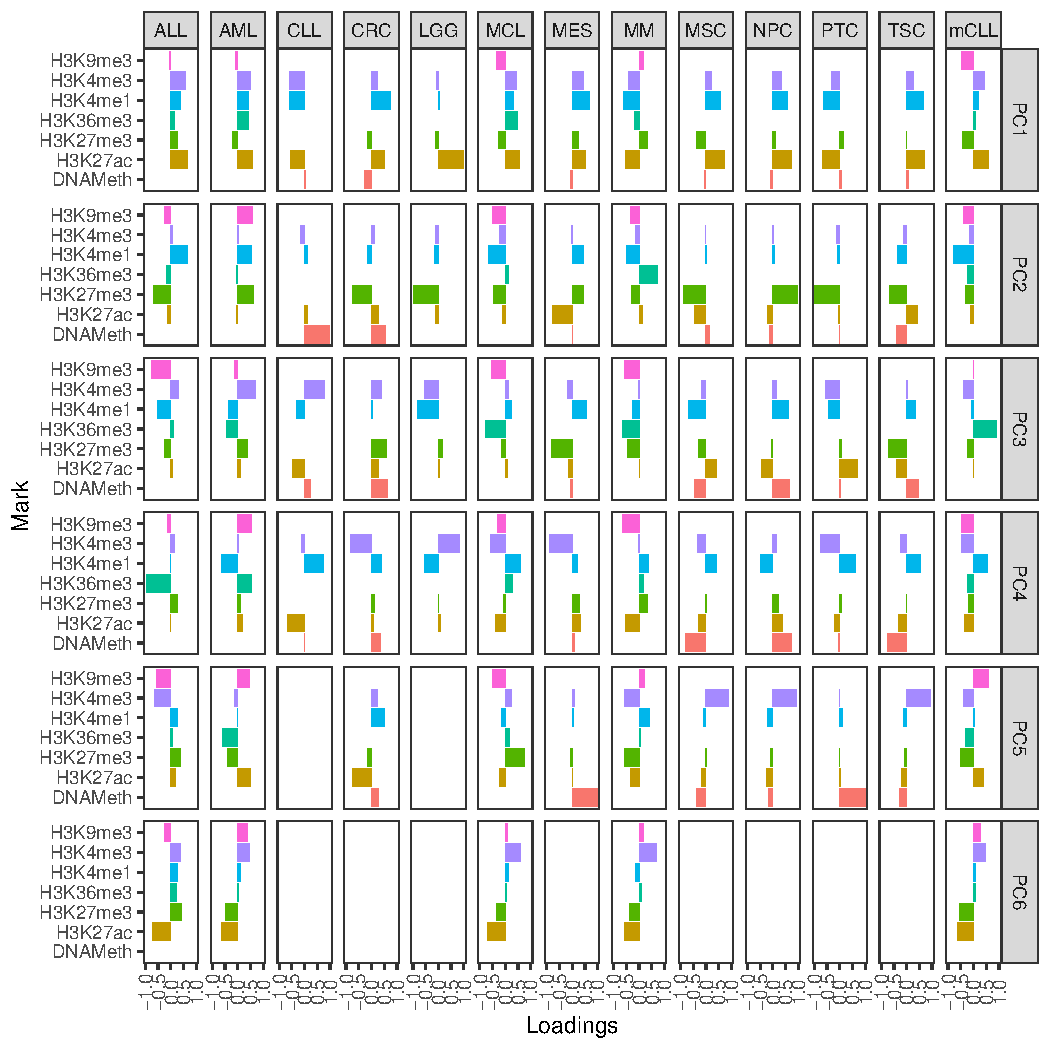
\includegraphics[scale=0.8]{figs/Loadings.pdf}
\caption{Histone mark contributions to each PC. PC1 appears to be mainly driven by active epigenetic marks}
\label{fig:pcload}
\end{figure}


\begin{figure}[!htb]
\centering
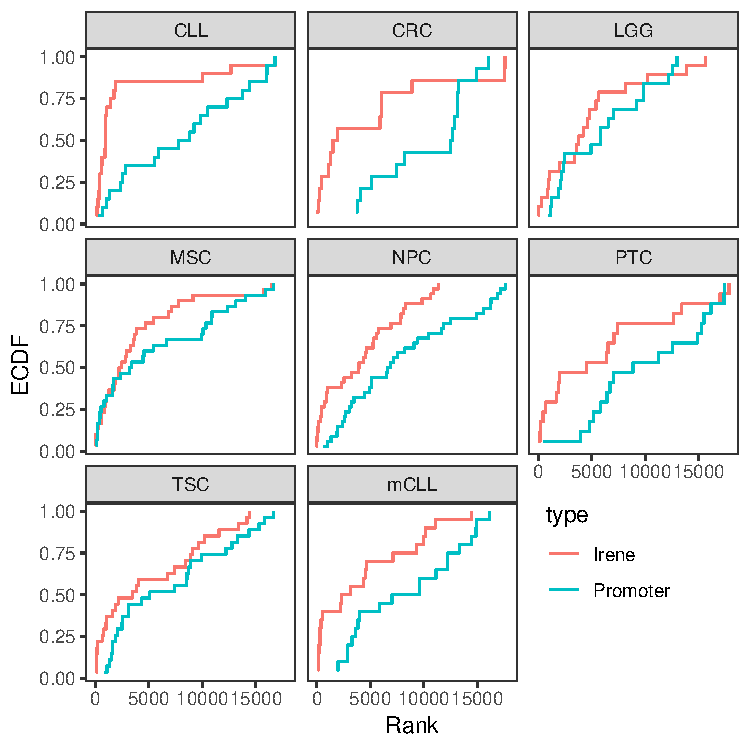
\includegraphics{figs/ROC.pdf}
\caption{ ROC of all test cases. Irene sorts the genes into descending order which is in accordance with the significance of alterations from both promoter and enhancers (aka "Irene" rank list), which is more relevant to the biological marker genes than the rank list derived from the PC1 order of only promoters (aka "Promoter" rank list).}
\label{fig:roc}
\end{figure}


\begin{figure}[!htb]
\centering
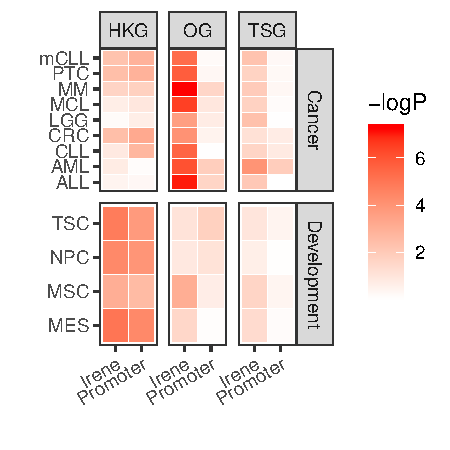
\includegraphics[scale=1.25]{figs/oncoRank.pdf}
\caption{ Wilcoxon-Mann-Whitney tests on the positions of oncogenes (OG), tumor suppressor genes (TSG), and housekeeping genes (HKG) in the {\em Irene} rank list against a uniformly distributed rank list of the same length. OGs in cancer are significantly ranked higher in {\em Irene} rank list, while they are not significant in developmental test cases. Moreover, all p-values are insignificant ($\geq 0.05$) when performed using {\em Promoter} rank list. }
\label{fig:og}
\end{figure}


\begin{figure}[!htb]
\centering
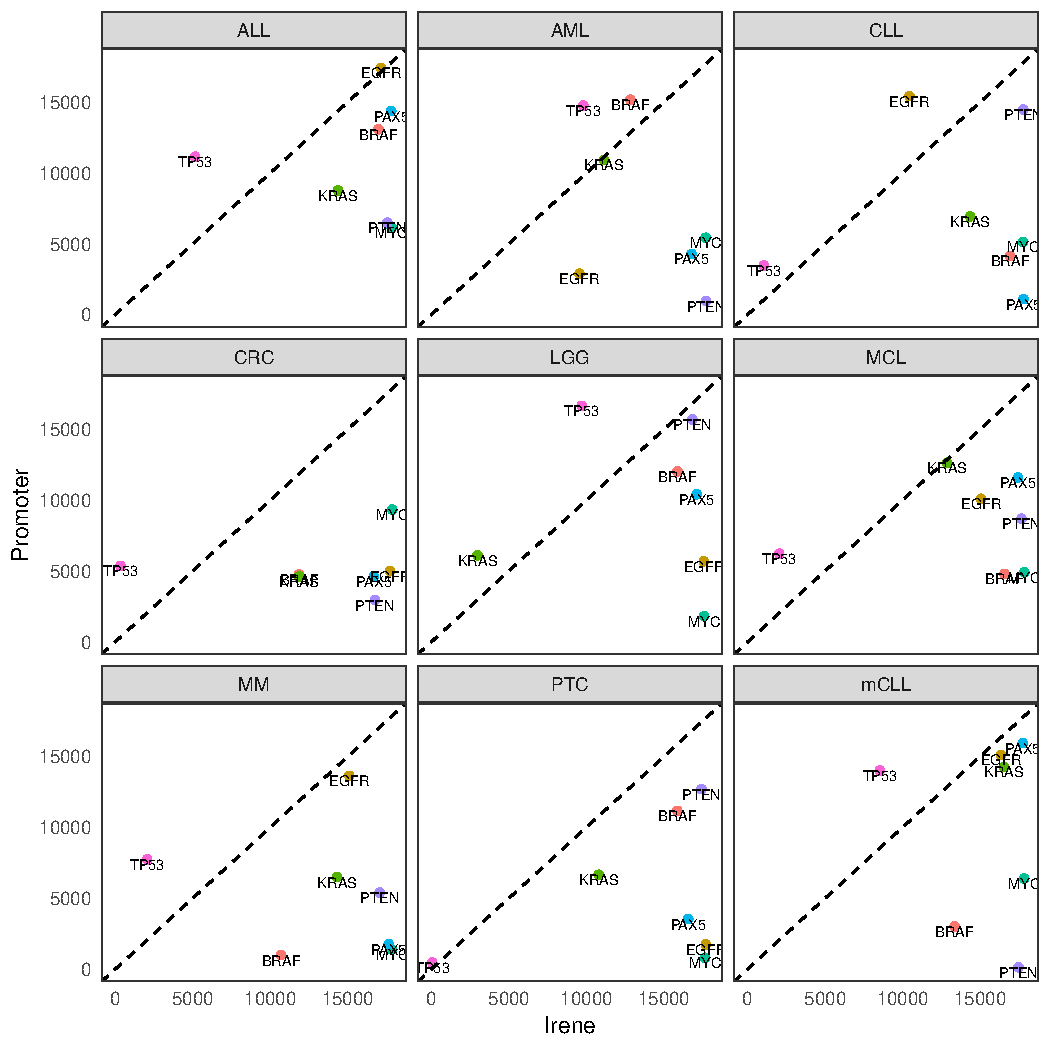
\includegraphics[scale=0.75]{figs/rnk.pdf}
\caption{ Ranking positions of well-known genes in {\em Irene} and {\em Promoter} list. Genes on the bottom-left corner are ranked worst in both lists, while genes on the top-right corner are ranked best in both lists. Genes on the top-left corner are only ranked best in {\em Promoter} list, and genes on bottom-right corner are only ranked best in {\em Irene} list. }
\label{fig:oncorank4}
\end{figure}


\begin{figure}[!htb]
\centering
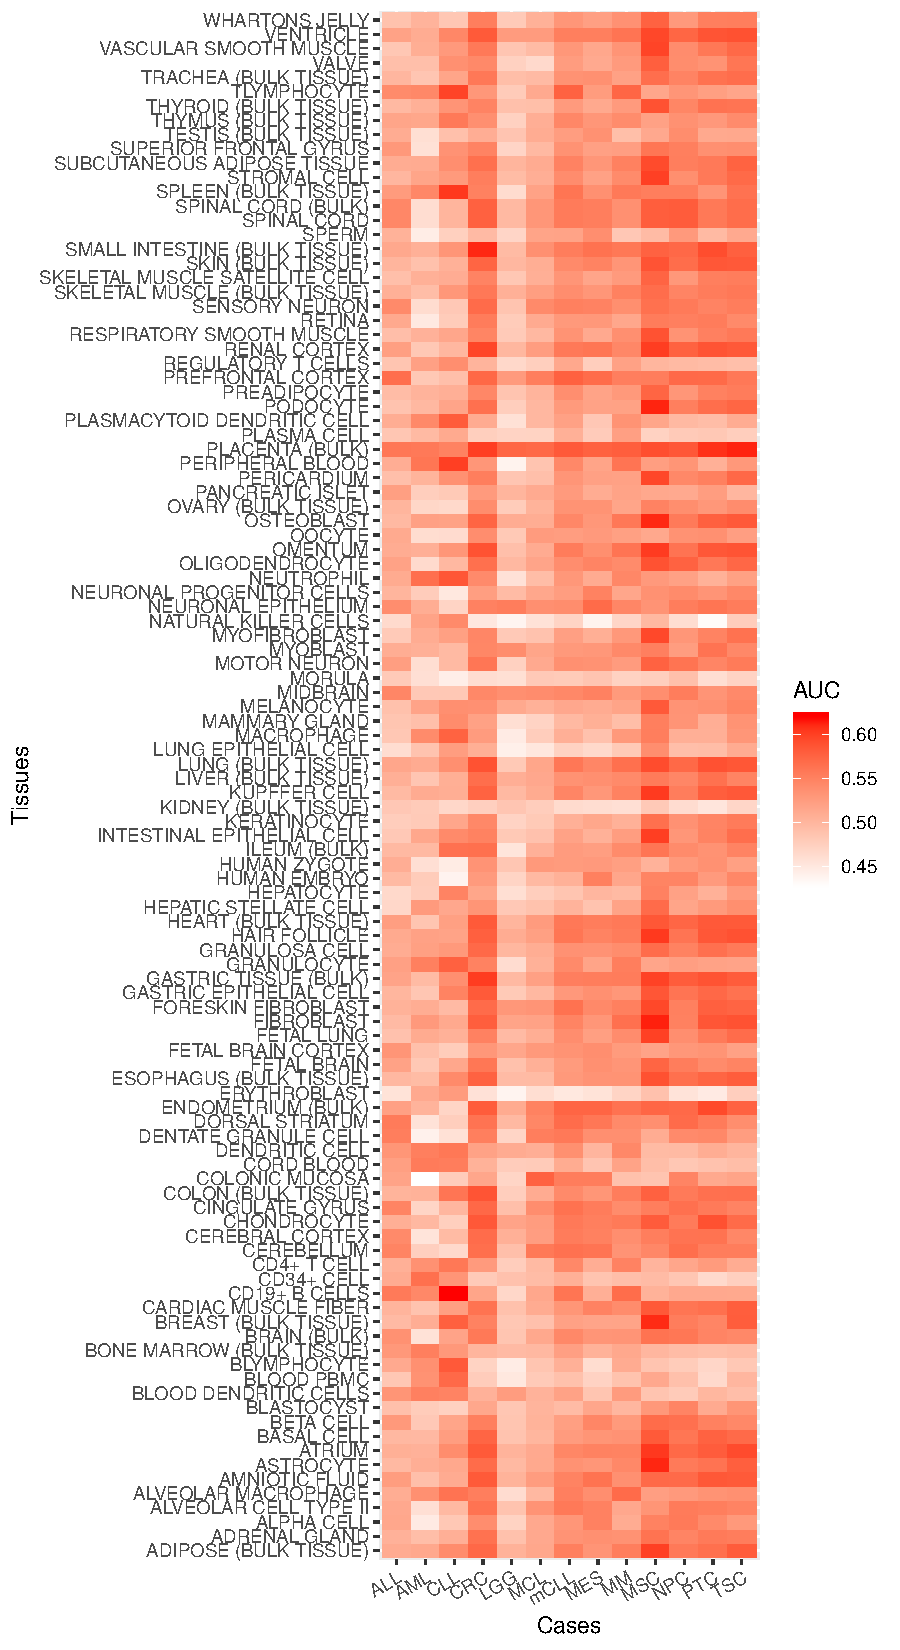
\includegraphics[scale=0.78]{figs/tissueAUC.pdf}
\caption{AUC differences between {\em Irene} rank and {\em promoter} rank of tissue specific genes, wherein we expected cancers have higher AUCs with respect to their tissues of origin, such as CRC with colon/intestine, B-cell neoplasms with blood cells, and PTC with thyroid, etc. }
\label{fig:rnd}
\end{figure}

\begin{figure}[!htb]
\centering
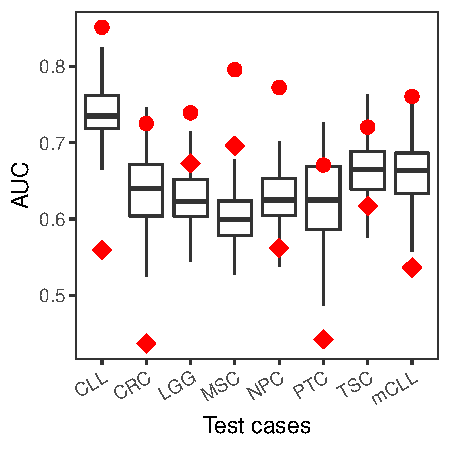
\includegraphics{figs/rnd.pdf}
\caption{AUCs of {\em Irene} rank from randomized promoter-enhancer interactions. The box plots indicate the quantile ranges from benchmarking each with 100 different rewired promoter-enhancer networks, whereas the red dots show the AUCs with the original promoter-enhancer interactions from {\em Irene} (in circles) and {\em Promoter} (in squares) rank lists. }
\label{fig:rnd}
\end{figure}

\begin{figure}[!htb]
\centering
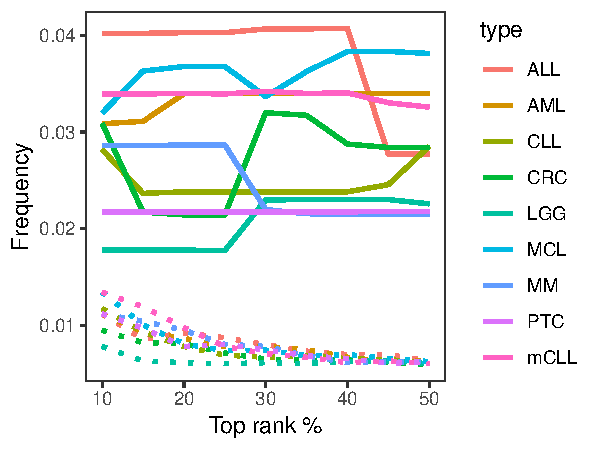
\includegraphics{figs/netRank.pdf}
\caption{Frequencies of oncogenes before/after the network clustering. The solid lines represent frequencies of oncogenes in the enriched subnetworks built from top 10\%-50\% genes of {\em Irene} rank list, while the dashed lines indicate the frequencies of oncogenes in the top 10\%-50\% of the {\em Irene} rank list. }
\label{fig:netrank}
\end{figure}


\begin{figure}[!htb]
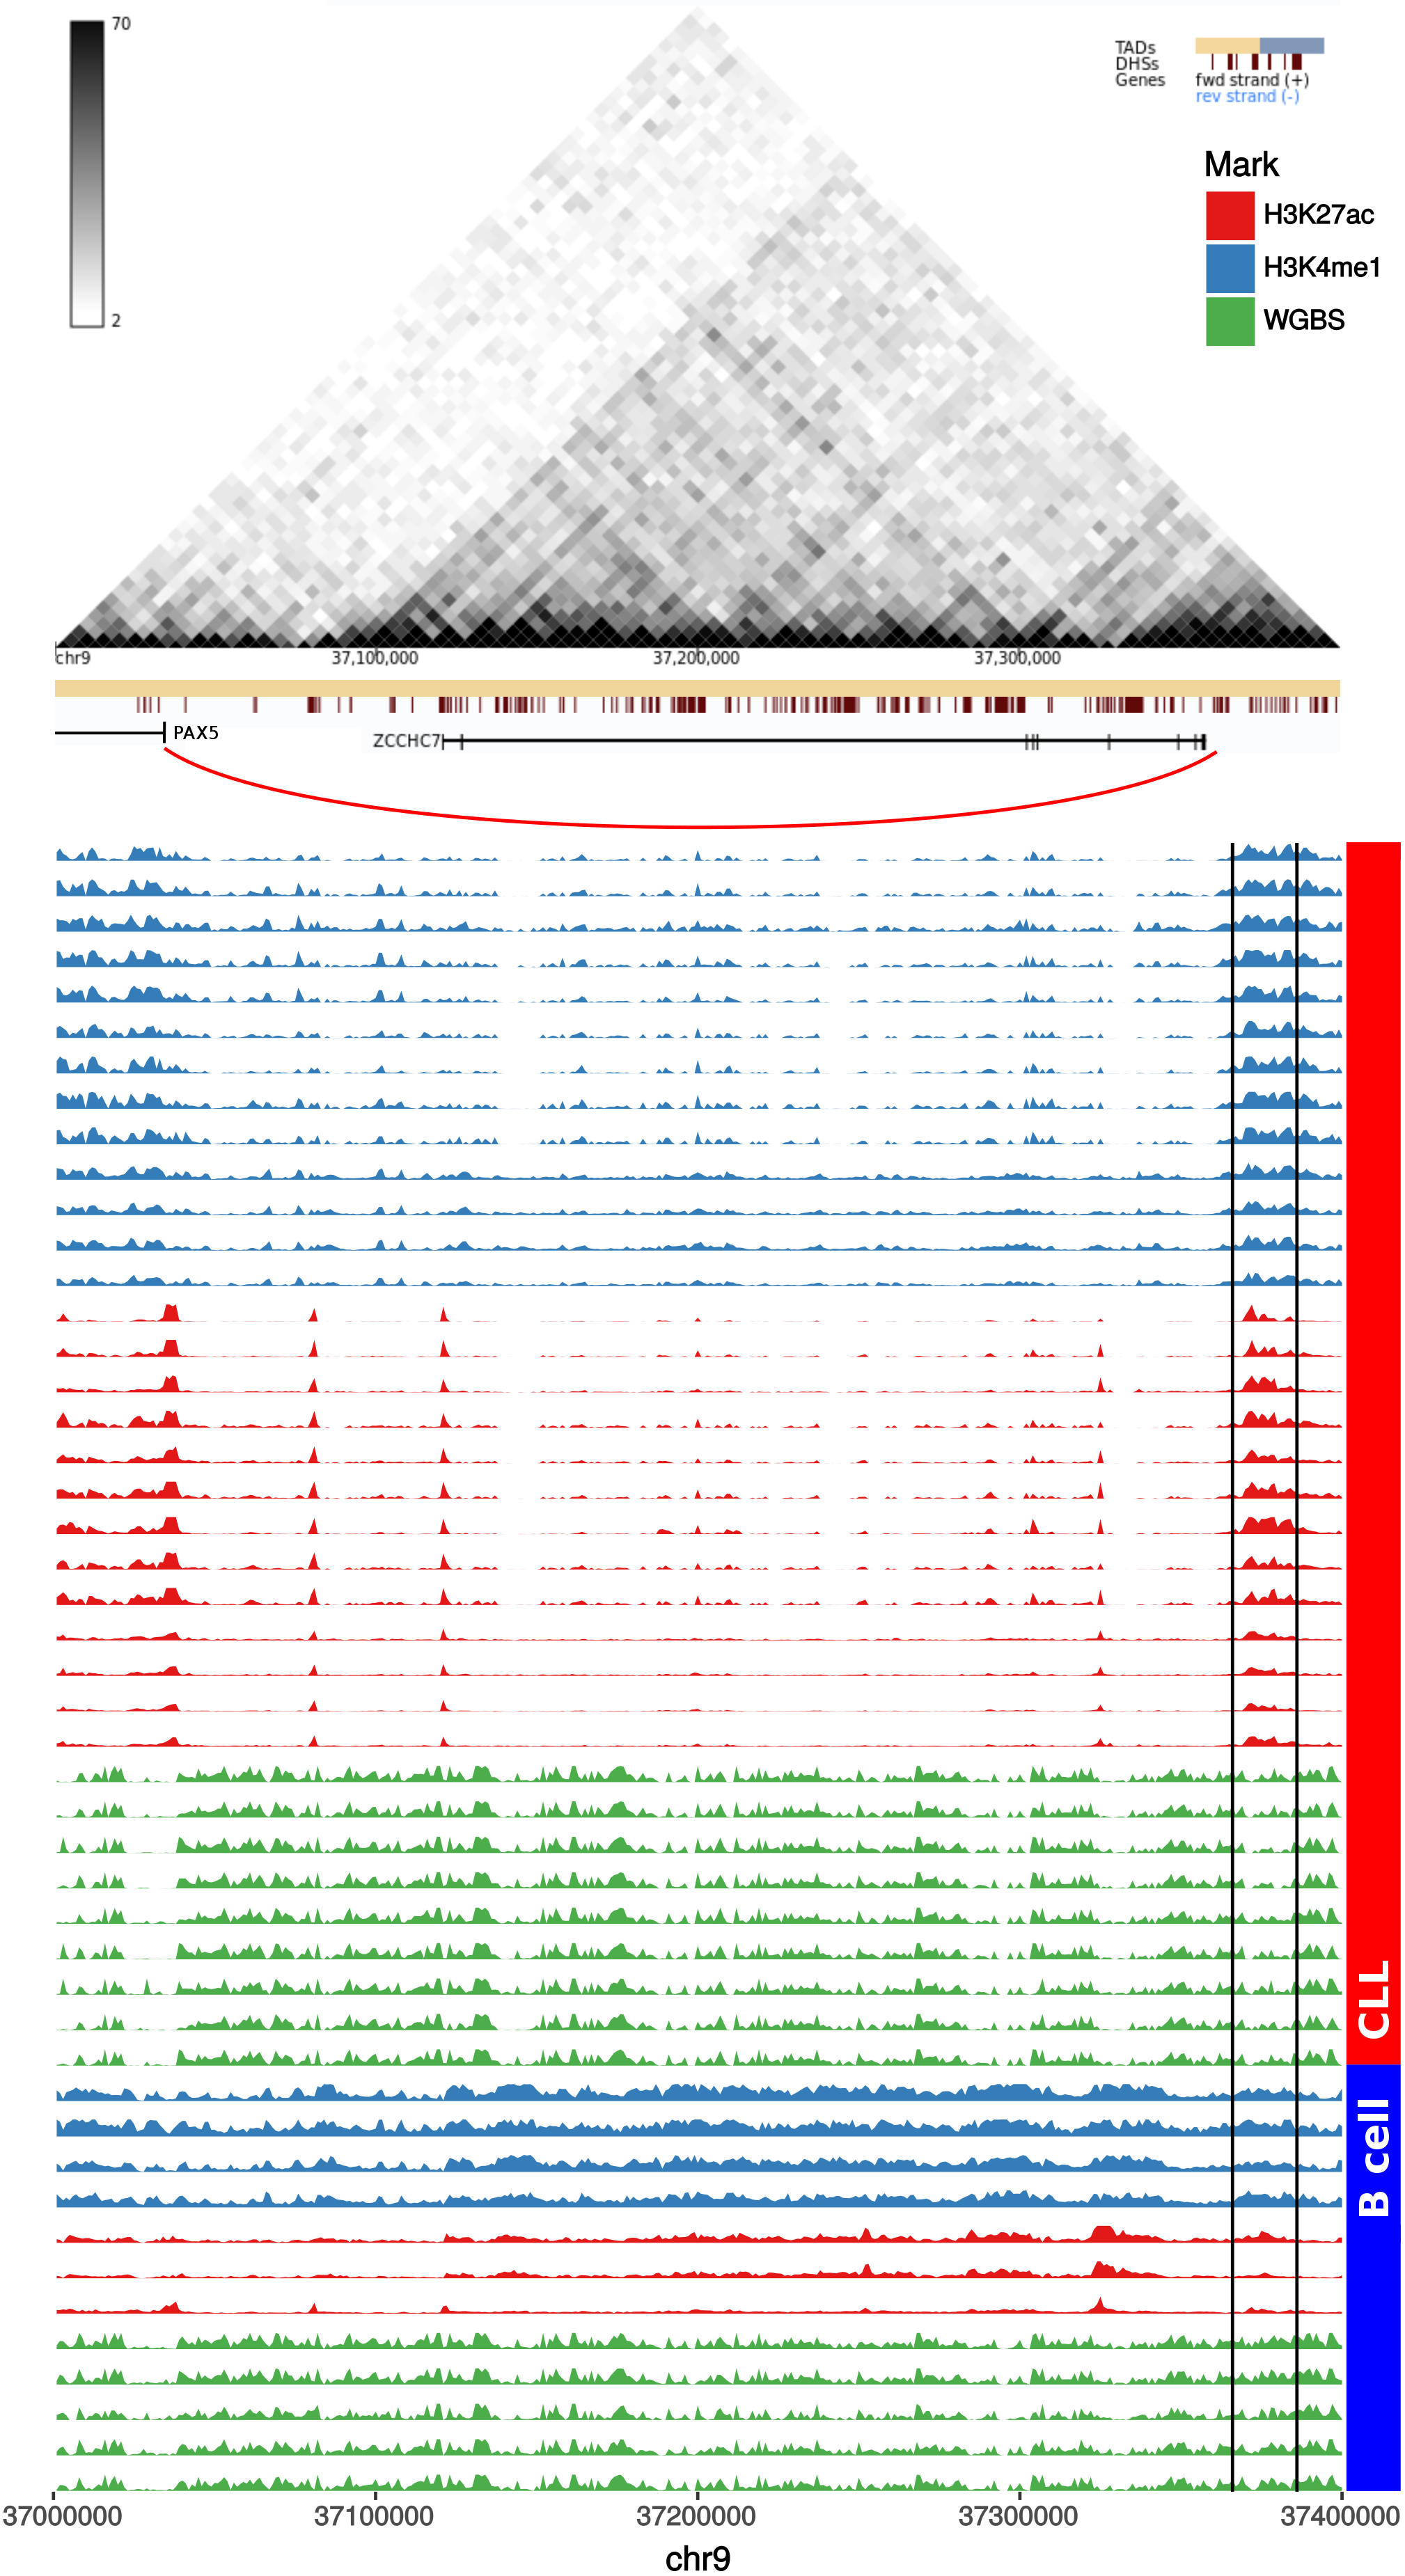
\includegraphics[scale=0.75]{figs/CLL-PAX5.pdf}
\caption{A known PAX5 enhancer in CLL exhibits hyperacetylation and hypomethylation. PAX5 promoter and enhancer are marked with grey shades, respectively. }
\label{fig:enhpax5}
\end{figure}
\end{document}